\documentclass[notitlepage]{article}
\usepackage{lmodern}
\usepackage[T1]{fontenc}
\usepackage[spanish]{babel}
\usepackage[utf8]{inputenc}
\usepackage{amsmath}
\usepackage{amsfonts}
\usepackage{mathtools}
\usepackage{amssymb}
\usepackage{amsthm}
\usepackage{enumerate}
\usepackage{hyperref}
\usepackage{graphicx}
\usepackage[document]{ragged2e}
\author{David Cardozo}
\title{Parcial de Probabilidad}
\theoremstyle{definition}
\newtheorem{defn}{Definición}[section]
\newtheorem{conj}{Conjetura}[section]
\newtheorem{exm}{Ejemplo}[section]
\theoremstyle{remark}
\newtheorem*{rem}{Observación}
\newtheorem*{note}{Nota}
\newtheorem{case}{Caso}
\newtheorem{exc}{Ejercicio}
\newtheorem*{sol}{Solución}

\newcommand{\pr}[1]{\mathbb{P}_{#1}}
\newcommand{\prob}[1]{\mathbb{P}(#1)}
\newcommand{\tq}{\text{ tal que }}
\newcommand{\lrp}[1]{\left( #1 \right)}
\newcommand{\abs}[1]{\left| #1 \right|}
\newcommand{\set}[1]{\left\lbrace #1 \right\rbrace}
\newcommand{\RR}{\mathbb{R}}
\newcommand{\CC}{\mathbb{C}}
\newcommand{\QQ}{\mathbb{Q}}
\newcommand{\ZZ}{\mathbb{Z}}
\newcommand{\R}{\mathbb{R}}
\newcommand{\N}{\mathbb{N}}
\newcommand{\ZN}[1]{\frac{\mathbb{Z}}{#1 \mathbb{Z}}}
\newcommand{\PP}{\mathbb{P}}
\newcommand{\qt}[1]{\textrm{#1}}
\newcommand{\function}[3]{#1 : #2 \rightarrow #3}
\newcommand{\contain}{\subseteq} %cambiar containded
\newcommand{\restric}[2]{ #1\restriction_{#2}}
\newcommand{\divs}{\mid}
\newcommand{\ndivs}{\nmid}
\newcommand{\paror}[1]{\big< #1 \big>}
\newcommand{\gothic}[1]{\mathfrak{#1}}

\begin{document}
	\maketitle
	\subsubsection*{Ejercicio 1}
	\begin{enumerate}[A)]
		\item \begin{enumerate}[1)]
			\item Sea $\mu_1$ una distribución en $\RR$. Calcule el parámetro $c \in \RR$ que falta.
			$$\mu_1(dx)= c \frac{1}{x}\mathbb{I}\{x>2 \}dx.$$
			\item Sea $\mu_2$ una distribución en $\R$. Calcule el parámetro $c \in \R$ que falta.
			$$\mu_2(dx)=5 \frac{1}{x^c}\mathbb{I}\{x>1 \}dx.$$
			\item Sea $\mu_3$ una distribución en $\R$. Calcule el parámetro $c \in \R$ que falta.
			$$\mu_3(dx)=5\frac{\log(x)}{x^c}\mathbb{I}\{x>1 \}dx.$$
			
		\end{enumerate}
		\item  Considere una familia independiente de variables aleatorias $(X_i)_{i\in \N}$, con $X_i\sim\mathcal{U}_{[0,1]}$.
		\begin{enumerate}[1)]
			\setcounter{enumii}{3}
			\item Calcule y dibuje la densidad de $X_1+X_2.$
			\item Calcule y dibuje la densidad de $X_1+X_2+X_3.$
			\item Calcule y dibuje la densidad de $X_1+X_2+X_2+X_4.$
			\item ¿Qué se puede decir de $\sum_{i=1}^{n}X_i$?
		\end{enumerate}
		\item Demuestre por cálculo directo que para las variables aleatorias $\perp(X,Y)$, se tienen las siguientes implicaciones:
		\begin{enumerate}[1)]
			\setcounter{enumii}{7}
			\item $X \sim \mathcal{P}_{\lambda}, Y \sim \mathcal{P}_{\lambda^{\prime}} \implies X+Y \sim \mathcal{P}_{\lambda+\lambda^\prime}.$
			\item $X \sim \mathcal{B}_{n_1,p}, Y \sim \mathcal{B}_{n_2,p} \implies X+Y \sim \mathcal{B}_{n_1+n_2,p}.$
			\item $X \sim N(m_1,\Omega_1^2), Y \sim N(m_2,\Omega_2^2)\implies$\\$ X+Y \sim N(m_1+m_2,\Omega_1^2+\Omega_2^2).$
		\end{enumerate} 
		
	\end{enumerate}	
	
	\subsubsection*{Solución 1}
	Para la solución de este ejercicio notamos que una distribución $ \mu $ aleatoria debe cumplir con la propiedad:
	\[ \int_{- \infty}^{\infty} \mu(dx) = 1  \]
	\begin{enumerate}[A)]
		\item \begin{enumerate}[1)]
			\item Observamos si tenemos una distribución:
			\begin{align*}
			\int_{-\infty}^{\infty} \mu_1(dx) = \int_{-\infty}^{\infty} c \cdot \frac{1}{x}\mathbb{I} \set{x > 2} dx  = 1 
			\end{align*}
			Solucionamos para calcular la constante:
			\begin{align*}
			1 = c \cdot \int_{2}^{\infty} \dfrac{dx}{x} \\
			\end{align*}
			y tenemos que esta integral no converge en $ (2,\infty) $, por lo cual concluimos que no existe $ c \in \RR $ para el cual $ \mu_1 $ sea una distribución de $ \RR $
			\item		Como en el punto anterior, si $ \mu_2(dx) $ es una distribución, debe cumplir que:
			\begin{align*}
			\int_{-\infty}^{\infty} \mu_2(dx) = \int_{- \infty}^{\infty} 5 \frac{1}{x^c} \mathbb{I}\set{x > 1}dx = 1 
			\end{align*}
			y obtenemos que:
			\begin{align*}
			1 &= 5 \cdot \int_{1}^{\infty}  \frac{dx}{x^c} \\
			&= \lim\limits_{t \rightarrow \infty} 5 \int_{1}^{t} \frac{1}{x^c} dx \\
			&= \lim\limits_{t \rightarrow \infty} 5 \lrp{\frac{x^{1-c}}{(1-c)}} \Big|_1^t \\
			&= \lim\limits_{t \rightarrow \infty} 5 \lrp{\frac{1}{c-1} - \frac{1}{(c-1)t^{c-1}}}
			\end{align*}
			evaluando, observamos que:
			\[ 1 = \frac{1}{c-1} \]
			y resolviendo para $ c $
			\[ c = 6 \]
			Concluimos que $ 6 $ es el valor adecuado para $ c $
			\item Observar que si $ c < 1 $ no es un valor adecuado, asumimos que $ c \geq 1 $
			\begin{eqnarray}
			\int_{-\infty}^{\infty}\mu_3(dx) &=& \int_{-\infty}^{\infty} 5\frac{\ln(x)}{x^c}\mathbb{I}\{x>1\}dx \nonumber = 1
			\\ 1 &=& \int_{1}^{\infty} 5\frac{\ln(x)}{x^c}dx \nonumber 
			\\ &=& \lim_{t \to \infty} \int_{1}^{t} 5\frac{\ln(x)}{x^c}dx \nonumber
			\end{eqnarray}
			Para evaluar esta integral, utilizamos integración por partes. Tomando:
			\[ u = \ln(x), dv = \frac{dx}{x^c} \]
			\begin{align*}
			\\ 1 =& \lim_{t \to \infty} 5\frac{\ln(x)}{(1-c)x^{c-1}}\bigg|_{1}^t - \int_{1}^{t} 5\frac{1}{(1-c)x^{c}}dx \nonumber 
			\\ =& \lim_{t \to \infty} 5\frac{\ln(x)}{(1-c)x^{c-1}}\bigg|_{1}^t - 5\frac{1}{(1-c)^2x^{c-1}} \bigg|_{1}^t \nonumber
			\\ =& \lim_{t \to \infty} 5\frac{\ln(t)}{(1-c)t^{c-1}}-5\frac{\ln(1)}{(1-c)1^{c-1}} - 5\frac{1}{(1-c)^2t^{c-1}}+5\frac{1}{(1-c)^21^{c-1}} \nonumber
			\\ =& \lim_{t \to \infty} \frac{5\ln(t)}{(1-c)t^{c-1}}- \frac{5}{(1-c)^2t^{c-1}}+\frac{5}{(1-c)^2} \nonumber
			\\ =& \frac{5}{(1-c)^2} +\lim_{t \to \infty} \frac{5\ln(t)}{(1-c)t^{c-1}}  \nonumber
			\end{align*}
			Para este ultimo limite, tomamos la regla de l'Hôpital para evaluarlo.
			\begin{align*}
			\\ 1 =& \frac{5}{(1-c)^2} +\lim_{t \to \infty} \frac{5\frac{1}{t}}{-(1-c)^2t^{c-2}} \nonumber
			\\ =& \frac{5}{(1-c)^2} +\lim_{t \to \infty} \frac{5}{-(1-c)^2t^{c-1}} \nonumber
			\\ =& \frac{5}{(1-c)^2} \nonumber
			\end{align*}
			Resolvemos 
			\[ (1-c^2) = 5 \]
			Recordando la restricción que $ c \geq 1 $, y concluimos que el parámetro  faltante es $ c = 1 + \sqrt{5} $
		\end{enumerate}
	\item 
		\begin{enumerate}[1)]
			\setcounter{enumii}{3}
			Recordamos que la densidad de la suma de variables independientes se calcula con la convolución de las densidades correspondientes
			\item Denotemos por $ f_i = \mathbb{I}\set{0 \leq x \leq 1} $ la función asociada a la variable $ X_i $. Denotemos por $ g $ función asociada a $ X_1 + X_2 $. tenemos:
			\begin{align*}
			g(x) &= \int_{\mathbb{R}} f_1(t)f_2(x-t)dt \nonumber
			\\g(x) &= \int_{\mathbb{R}} \mathbb{I}\{0 \leq t \leq 1\}\mathbb{I}\{0 \leq x-t \leq 1\}dt
			\end{align*}
			ambas por definición. Partimos las integrales en casos y obtenemos:
			\[ g(x)= \int_{\mathbb{R}} \mathbb{I}\{0 \leq t \leq 1\}\mathbb{I}\{0 \leq x-t \leq 1\}dt = \int_0^x dt = t\bigg|_0^x=x \]
			para $ 0 \leq x \leq 1 $
			y 
			\[ g(x)= \int_{\mathbb{R}} \mathbb{I}\{0 \leq t \leq 1\}\mathbb{I}\{0 \leq x-t \leq 1\}dt = \int_x-1^1 dt = t\bigg|_{x-1}^1=2-x  \]
			para $ 1 \leq x \leq 2 $.
			Combinando estos resultados obtenemos la gráfica:
			\[ 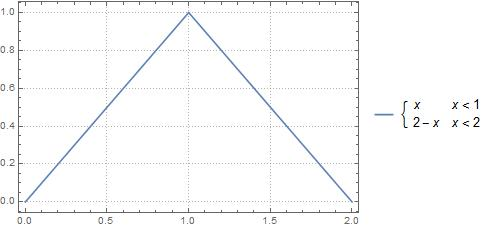
\includegraphics[scale=0.5]{Graph1.jpg} \]
			
			\item Similarmente como en el punto anterior hacemos la convolución correspondiente (teniendo en cuenta que ya tenemos $ X_1 + X_2 $) tomamos:
			\[ h(x)=\int_{\mathbb{R}} g(t)f_3(x-t)dt \]
			utilizando el punto anterior y las definiciones correspondientes de cada función, tenemos:
			\[ h(x) = \int_{\mathbb{R}} t\cdot\mathbb{I}\{0\leq t \leq 1\}\mathbb{I}\{0 \leq x-t \leq 1\}dt + \int_{\mathbb{R}} (2-t)\cdot \mathbb{I}\{1\leq t \leq 2\}\mathbb{I}\{0 \leq x-t \leq 1\}dt \]
			Similar al anterior partimos por casos, y obtenemos(Integrales calculadas mediante Mathematica\textregistered):
			\[ h(x) = \begin{cases}
			\frac{x^2}{2} & \textrm{si } 0 \leq x < 1 \\
			-x^2 + 3x - \frac{3}{2} & \textrm{si } 1 \leq x < 2 \\
			\frac{x^2}{2} - 3x + \frac{9}{2} & \textrm{si } 2 \leq x \leq 3
			\end{cases} \]
			y su gráfica corresponde a:
			\[ 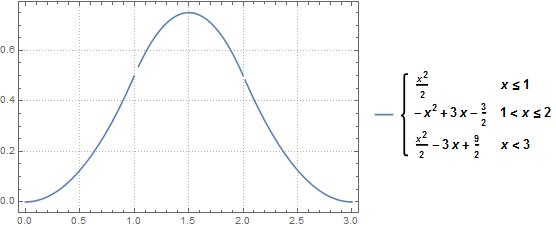
\includegraphics[scale=0.5]{Graph2.jpg} \]
			\item Tomamos información de los items anteriores y definimos:
			\[ l(x) = \int_{\mathbb{R}} h(x)f_4(x-t)dt  \]
			y encontramos que esta función esta dada por:
			\begin{equation*}
			\begin{multlined}
			l(x) = \int_{\mathbb{R}} \mathbb{I}\{0\leq t \leq 1\}\mathbb{I}\{0\leq x-t \leq 1\}\frac{t^2}{2}dt + \int_{\mathbb{R}} \mathbb{I}\{1\leq t \leq 2\}\mathbb{I}\{0\leq x-t \leq 1\}(-t^2+3t-\frac{3}{2})dt \\
		 + \int_{\mathbb{R}} \mathbb{I}\{2\leq t \leq 3\}\mathbb{I}\{0\leq x-t \leq 1\}(\frac{t^2}{2}-3t+\frac{9}{2})dt 
			\end{multlined}
			\end{equation*}
		
		\item En lo mismo que en los anteriores casos, partimos y analizamos casos, el procedimiento de calculo se realiza con la ayuda de Mathematica, y no se transcribe debido a no realizar el trabajo muy extenso. Concluimos que:
		\[ l(x) = \begin{cases}
		\frac{x^3}{6}  & \text{si } 0 \leq x < 1 \\
		-\frac{x^3}{2}+2x^2-2x+\frac{2}{3} & \textrm{si } 1 \leq x < 2 \\
		\frac{x^3}{2}-4x^2+10x-\frac{22}{3} & \textrm{si } 2 < x\leq 3 \\
		-\frac{x^3}{6}+2x^2-8x+\frac{32}{3} & \textrm{si } 3 <  x\leq 4
		\end{cases} \]
		\[ 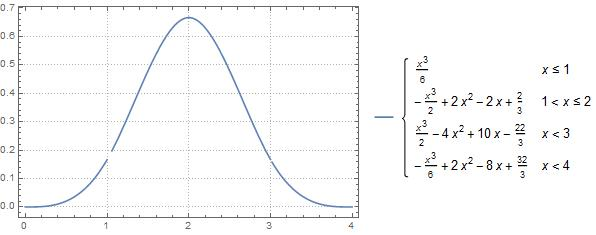
\includegraphics[scale=0.5]{Graph3} \]
		\item Hay varias características que podemos notar, gracias a las propiedades de la integración y las gráficas adjuntas, podemos conjeturar las siguientes características de como sería $ \sum X_i $ :
		\begin{enumerate}
			\item Obtiene valor máximo en la mitad del intervalo $ n/2 $
			\item Se parece cada vez mas y mas a $ \mathcal{B}_{n, \frac{1}{2}} $ 
		\end{enumerate}
		Se esperaría que exista una formula cerrada para el n-esímo valor, pero podría ser falso que fuera una función corta y sencilla.
	\end{enumerate}
		\item 
			\begin{enumerate}[1)]
				\setcounter{enumii}{7}
				\item $X \sim \mathcal{P}_{\lambda}, Y \sim \mathcal{P}_{\lambda^{\prime}} \implies X+Y \sim \mathcal{P}_{\lambda+\lambda^\prime}.$
				\begin{proof}
					Sean $ X,Y $ variables aleatorias, sabemos que si $ f,g $ son las funciones de masa asociadas a $ X,Y $, la función masa de $ X + Y $ esta dada por:
					\[ s(x) = \sum_{t=0}^x f(t)g(x-t) \]
					Sabemos que para Poission las funciones son dadas por:
					\[ f(x) = \frac{e^{-\lambda}\lambda^x}{x!}  \]
					y 
					\[   g(x) = \frac{e^{-\lambda'}(\lambda')^x}{x!} \]
					Utilizando la primera formula, remplazando valores tenemos:
					\[ s(x) =  \sum_{t=0}^x \frac{e^{-\lambda}\lambda^t}{t!}\frac{e^{-\lambda'}(\lambda')^{x-t}}{(x-t)!}  \]
					reorganizando:
					\[ s(x) = e^{-(\lambda+\lambda')}\sum_{t=0}^x\frac{\lambda^t(\lambda')^{x-t}}{t!(x-t)!} \]
					Por lo tanto:
					\[ s(x) = e^{-(\lambda+\lambda')}\sum_{t=0}^x\frac{\lambda^t(\lambda')^{x-t}}{t!(x-t)!} \]
					Identificamos en esta expresión el coeficiente binomial, y tenemos que:
					\[ s(x)= e^{-(\lambda+\lambda')}\sum_{t=0}^x \frac{1}{x!}\binom{x}{t}\lambda^t(\lambda')^{x-t} \]
					\[s(x) = \frac{e^{{-(\lambda+\lambda')}}}{x!}\sum_{t=0}^x \binom{x}{t}\lambda^t(\lambda')^{x-t} \]
					como $ x $ es entero, identificamos que:
					\[ (\lambda + \lambda')^x =  \sum_{t=0}^x \binom{x}{t}\lambda^t(\lambda')^{x-t}  \]
					y finalmente:
					\[ s(x) =  \frac{e^{-(\lambda+\lambda')}(\lambda+\lambda')^x}{x!}  \]
				\end{proof}
				\item $X \sim \mathcal{B}_{n_1,p}, Y \sim \mathcal{B}_{n_2,p} \implies X+Y \sim \mathcal{B}_{n_1+n_2,p}.$
				\begin{proof}
					Similar al punto anterior, definimos ahora X,Y funciones aleatorias con funciones asociadas:
					\[ f(x) =  \binom{n_1}{x}p^x(1-p)^{n_1-x} \]
					y \[ g(x) = \binom{n_2}{x}p^x(1-p)^{n_2-x} \]
					ahora recordemos:
					\[  s(x) = \sum_{t=0}^x f(t)g(x-t) \]
					remplazando, por sus definiciones, tenemos:
					\begin{align*}
					s(x) &= \sum_{t=0}^x \binom{n_1}{t}\binom{n_2}{x-t}p^{t+x-t}(1-p)^{n_1-t+n_2-(x-t)}  \\
					&= p^{x}(1-p)^{n_1+n_2-x}  \sum_{t=0}^x \binom{n_1}{t}\binom{n_2}{x-t}
					\end{align*} 
					Como queremos llegar a una factorización de la forma $ (x+1)^{n_1} (x+1)^{n_2}$, podemos utilizar el producto de Cauchy. Tenemos entonces:
					\[ \binom{n_1 + n_2}{x} = \sum_{t=0}^x \binom{n_1}{t} \cdot \binom{n_2}{x-t} \]
					Lo cual directamente lleva a que podemos escribir $ s $ de la forma:
					\[ s(x) = p^{x}(1-p)^{n_1+n_2-x}  \sum_{t=0}^x \binom{n_1}{t}\binom{n_2}{x-t} = \binom{n_1+n_2}{x} p^{x}(1-p)^{n_1+n_2-x} \]
					hemos mostrado por calculo directo que $  X+Y \sim \mathcal{B}_{n_1+n_2,p}.$ 
				\end{proof}
				\end{enumerate} 
	
	\end{enumerate}
	

	
	
	\subsubsection*{Ejercicio 2}
		En un típico texto alemán, la letra e es la más frecuente con un $12.5$ \% de probabilidad, por encima de todas las demás letras. Un software reapasa un texto desconocido de una forma puramente aleatoria y reconoce con $99$\% de la letra e correctamente. Con la probabilidad de $0.1$\% reconoce una e erroneamente.
		\begin{enumerate}[1.]
			\item ¿Qué tan grande es la probabilidad de que el softaware indique la letra e en un paso?
			\item ¿Qué tan grande es la probabilidad de que sea efectivamente la letra e cuando detecta una e?\\			
		\end{enumerate}
		\textit{Formalice estas probabilidades y cuide meticulosamente la notación.\\
			Identifique todos los eventos que utiliza.\\
			Calcule todo en fracciones y de el resultado como fracción simplificada de dos números enteros.}
		
	\subsubsection*{Solución 2}
		\begin{enumerate}[1.]
		\item Modelizamos de la forma \[ \set{E,NE} \times \set{ De,NDe }  \], donde $ E $ es leer la letra $ e $, $ NE $, no leer la letra $ e $, $ De $ es detectar una $ e $ y por ultimo $ NDe $ es no detectar una $ e $. Naturalmente los estados serían: \[ A = \set{(E, De), (E, NDe)} \] y \[ B = \set{(E,De),(NE,De)} \]
		Las siguientes son las probabilidades dadas:
		\[ \PP(A) = \frac{1}{8} \quad \PP(A^C) = \frac{7}{8} \quad \PP(B|A) = \frac{99}{100} \quad \PP(B|A^C) = \frac{1}{1000}  \]
		Por lo tanto si queremos calcular $ \PP(B) $
		\[ \mathbb{P}(B)=\prob{A}\mathbb{P}(B|A)+\prob{A^C}\prob{B|A^C} = \frac{10019}{80000} \]
		\item Fácilmente usando Bayes:
		\[ \prob{A|B} = \frac{\prob{B|A}\prob{A}}{\prob{B}} = \frac{9900}{10019}  \]
		\end{enumerate}	
	
	
	\subsubsection*{Ejercicio 3}
	\textbf{Sin memoria implica distribución exponencial o geométrica.}
	\begin{enumerate}[1)]
		\item Demuestre que para toda variable aleatoria con valores $[0,\infty)$ cuya distribución $\mathbb{P}_X$ es absolutamente contínua con respecto a la medida de Lebesgue, con una densidad estrictamente positiva y que satisface:
		$$\forall t,s>0, 0< \mathbb{P}(X>t+s\vert X>t)=\mathbb{P}(X>s)<1.$$
		Se tiene que $\exists \lambda >0 \tq \mathbb{P}_X=\exp(\lambda)$.
		\\ \textit{Ayuda: Calcule la ecuación que satisface $\log(1-F_X)$, resuelva la ecuación y deduzca el resultado.}
		\item Demuestre que para toda variable aleatoria $X$ con valores en $\N$, cuya distribucion $\mathbb{P}_X$ satisface:
		$$\mathbb{P}(X>n+m\vert X>m)=\mathbb{P}(X>n), \forall n,m \in \N\backslash{0}.$$
		Se tiene que existe un parámetro $a \in (0,1]$ tal que $X \sim \mathcal{G}_a$.
	
		\end{enumerate}
			\textit{Ayuda: Calcule $\mathbb{P} (x = k)$ como diferencia de $1$ menos la función de distribución y use el inciso anterior. La demostración se hace entonces, por inducción}
			
		\begin{sol}
			\begin{enumerate}
			\item
			Suponga que la distribución $ \mathbb{P}_X $ es absolutamente contínua con respecto a la medida de Lebesgue, y se cumple:
			\[ \forall t,s>0, 0< \mathbb{P}(X>t+s\vert X>t)=\mathbb{P}(X>s)<1  \]
			sabemos que:
			\[ \PP\lrp{x > t + s | x \geq t} = \frac{P(x > t + s)}{\PP(x > t)} = P(x > s) \]
			es decir:
			\[ \PP(x > t + s) = \PP(x > s)\PP(x > t) \]
			y sabemos que $ F_x(t + s) = \PP(x \leq t +s) $
			\[ 1 - F(t + s) = \left\lbrack 1 - F(s) \right\rbrack \left\lbrack 1 - F(t) \right\rbrace  \]
			\[ G(t +s) = G(s)G(t) \]
			\[ G(x) = G(1)G(x-1) \]
			\[ G(x) = \left\lbrack G(1) \right\rbrack^x\]
			\[ \ln(G(x)) = x \ln G(1) \]
			\[ \ln(1-F(x)) = x \ln(1 - F(1)) \]
			y definamos ahora:
			\[ \lambda = - \ln(1 - F(1)) \]
			Si procedemos a sacar exponentes a ambos lados de la ecuación, terminamos con:
			\[ 1- F(x) = e^{-\lambda x} \]
			\[ F(x) = 1 - e^{-\lambda x} \]
			y podemos calcular $ f $ gracias a $ f = F' $
			\[ f(x) = \lambda e^{-\lambda x} \]
			que es la función densidad  de distribucion, exponencial
			\item
			Similarmente al anterior,
			\begin{equation}
			\prob{X>n}\prob{X>m}=\prob{X>n+m} \nonumber
			\end{equation}
			 $ \prob{X>x}=1-\prob{X\leq x} 1-\sum_{i=1}^x \prob{X=i} $, y terminamos con
			
			\begin{equation}
			(1-\sum_{i=1}^n \prob{X=i})(1-\sum_{i=1}^m \prob{X=i})=(1-\sum_{i=1}^{n+m} \prob{X=i}) \nonumber
			\end{equation}
			
			Queremos ver:
			\begin{equation}
			(1-\sum_{i=1}^x \prob{X=i}) = q^x
			\end{equation}
			
			para algún $ q \in \mathbb{R} $.
			
			Procedamos por inducción:
			
			\textbf{Caso Base} \[ 1-\sum_{i=1}^1 \prob{X=i} = 1-\prob{X=1 }\]. Vemos $ q = 1-\prob{X=1} $ ya cumple la condición
			
			Por hipótesis $ \forall x>1  $, se cumple que $\displaystyle 1-\sum_{i=1}^x \prob{X = i} = (1-\sum_{i=1}^n \prob{X=i})(1-\sum_{i=1}^m \prob{X=i}) $. 
			
			\textbf{Hipótesis de Inducción}  $ \displaystyle 1-\sum_{i=1}^x \prob{X = i} = q^nq^m=q^{n+m}= q^x $.
			
			Y podemos entonces:
			\begin{equation}
			\prob{X=x}= 1-\sum_{i=1}^{x-1}\prob{X=i}-(1-\sum_{i=1}^{x} \prob{X=i}) = q^{x-1}-q^{x} = q^{x-1}(1-q). \nonumber
			\end{equation}
			
			Concluimos entonces que $ \sum_{i=1}^\infty \prob{X=i} = (1-q)\sum_{i=1}^\infty q^{x-1} $ debe converger y debe ser mayor que 0. Por lo tanto, como esta es la serie geométrica tenemos que $ 0 \leq q < 1 $. Por ultimo si tomamos $ p = 1- q $ tendríamos que $ \prob{X=x} = p(1-p)^{x-1} $ con $ 0<p\leq 1 $ y esta es la distribución geométrica con parámetro $ p $
		\end{enumerate}
		\end{sol}
		
	
	\subsubsection*{Ejercicio 4}
	
	\begin{enumerate}[1)]
		\item Sea $ X = (X_1,X_2): \Omega \rightarrow \set{0,1,2}^2 $ es un vector aleatorio con marginales:
		\begin{align*}
		\mathbb{P}_{X_1} = \alpha_0\delta_0 + \alpha_1\delta_1 + \alpha_2\delta_2 \\
		\mathbb{P}_{X_2} = \beta_0\delta_0 + \beta_1\delta_1 + \beta_2\delta_2
		\end{align*}
		Construya el sistema lineal de todas las ecuaciones y reduzcalo lo máximo posible con el algoritmo de Gauss. Cuántos grados de libertad existen para estas leyes de $ \mathbb{P}_X $ en el espacio producto $ \set{0,1,2}^2 $
		\item Sea $ X = \lrp{X_1, X_2, X_3}: \Omega \rightarrow \set{0,1}^3 $ un vector aleatorio con marginales:
		\begin{align*}
		\mathbb{P}_{X_1} = \alpha_0\delta_0 + \alpha_1\delta_1, \\
		\mathbb{P}_{X_2} = \beta_0\delta_0 + \beta_1\delta_1, \\
		\mathbb{P}_{X_3} = \gamma_0\delta_0 + \gamma_1\delta_1.
		\end{align*}
		Construya el sistema lineal de todas las ecuaciones y reduzcalo lo máximo posible con el algoritmo de Gauss. Cuántos grados de libertad existen para estas leyes de $ \mathbb{P}_X $ en el espacio producto $ \set{0,1}^3 $ ?
		\item Sea $ X = \lrp{X_1,X_2,X_3}: \Omega \rightarrow \set{0,1}^3 $ un vector aleatorio con los marginales:
		\[ \mathbb{P}_{\lrp{X_1,X_2}} = \mathbb{P}_{X_1,X_3} = \mathbb{P}_{X_2,X_3} = \beta_{00}\delta_{\lrp{00}} + \beta_{01}\delta_{\lrp{0,1}} + \beta_{10}\delta_{lrp{1,0}} + \delta_{11}\delta_{\lrp{1,1}}. \]
		Construya el sistema lineal de todas las ecuaciones y reduzcalo lo máximo posible con el algoritmo de Gauss. Cuántos grados de libertad existen para estas leyes de $ \mathbb{P}_X $ en el espacio producto $ \set{0,1}^3 $?
	\end{enumerate}
	
	\subsubsection*{Solución 4}
	\begin{itemize}
		\item Construya el sistema lineal de todas las ecuaciones y reduzcalo lo máximo posible con el algoritmo de Gauss. Cuántos grados de libertad existen para estas leyes de $ \mathbb{P}_X $ en el espacio producto $ \{0,1,2\}^2 $?
		\begin{sol}
			Considere $ \pr{ij}=\prob{X_1=i \cap X_2 = j} $. y observamos que deben cumplir:
			
			\begin{eqnarray}
			\alpha_0 &=&\pr{00}+\pr{01}+\pr{02} \nonumber
			\\\alpha_1 &=& \pr{10}+\pr{11}+\pr{12} \nonumber
			\\\alpha_2 &=& \pr{20}+\pr{21}+\pr{22} \nonumber
			\\\beta_0 &=& \pr{00}+\pr{10}+\pr{20} \nonumber
			\\\beta_1 &=& \pr{01}+\pr{11}+\pr{21} \nonumber
			\\\beta_2 &=& \pr{02}+\pr{12}+\pr{22} \nonumber
			\end{eqnarray}
			
			Y este sistema lo podemos ver en la matriz:
			\begin{equation}
			\begin{pmatrix}
			1 & 1 & 1 & 0 & 0 & 0 & 0 & 0 & 0
			\\0 & 0 & 0 & 1 & 1 & 1 & 0 & 0 & 0
			\\0 & 0 & 0 & 0 & 0 & 0 & 1 & 1 & 1
			\\1 & 0 & 0 & 1 & 0 & 0 & 1 & 0 & 0
			\\0 & 1 & 0 & 0 & 1 & 0 & 0 & 1 & 0
			\\0 & 0 & 1 & 0 & 0 & 1 & 0 & 0 & 1
			\end{pmatrix} \nonumber
			\end{equation}
			Utilizando \textit{Row Reduce} con Mathematica obtenemos que:
			\begin{equation}
			\begin{pmatrix}
			1 & 0 & 0 & 0 & -1 & -1 & 0 & -1 & -1 \\
			0 & 1 & 0 & 0 & 1 & 0 & 0 & 1 & 0 \\
			0 & 0 & 1 & 0 & 0 & 1 & 0 & 0 & 1 \\
			0 & 0 & 0 & 1 & 1 & 1 & 0 & 0 & 0 \\
			0 & 0 & 0 & 0 & 0 & 0 & 1 & 1 & 1 \\
			0 & 0 & 0 & 0 & 0 & 0 & 0 & 0 & 0
			\end{pmatrix} \nonumber
			\end{equation}
			Concluimos entonces que hay 5 grados de libertad
		\end{sol}
		\item
		\begin{sol}
			Similar al ejercicio anterior, formamos la tabla asociada: 
			\begin{eqnarray}
			\alpha_0 &=& \pr{000}+\pr{001}+\pr{010}+\pr{011} \nonumber
			\\\alpha_1 &=& \pr{100}+\pr{101}+\pr{110}+\pr{111} \nonumber
			\\\beta_0 &=& \pr{000}+\pr{001}+\pr{100}+\pr{101} \nonumber
			\\\beta_1 &=& \pr{010}+\pr{011}+\pr{110}+\pr{111} \nonumber
			\\\gamma_0 &=& \pr{000}+\pr{010}+\pr{100}+\pr{110} \nonumber
			\\\gamma_1 &=& \pr{001}+\pr{011}+\pr{101}+\pr{111} \nonumber
			\end{eqnarray}
			
			Con matriz:
			\begin{equation}
			\begin{pmatrix}
			1 & 1 & 1 & 1 & 0 & 0 & 0 & 0 \\
			0 & 0 & 0 & 0 & 1 & 1 & 1 & 1 \\
			1 & 1 & 0 & 0 & 1 & 1 & 0 & 0 \\
			0 & 0 & 1 & 1 & 0 & 0 & 1 & 1 \\
			1 & 0 & 1 & 0 & 1 & 0 & 1 & 0 \\
			0 & 1 & 0 & 1 & 0 & 1 & 0 & 1
			\end{pmatrix}\nonumber
			\end{equation}
			
			Utilizando \textit{Row Reduce} con Mathematica obtenemos que:
			\begin{equation}
			\begin{pmatrix}
			1 & 0 & 0 & -1 & 0 & -1 & -1 & -2 \\
			0 & 1 & 0 & 1 & 0 & 1 & 0 & 1 \\
			0 & 0 & 1 & 1 & 0 & 0 & 1 & 1 \\
			0 & 0 & 0 & 0 & 1 & 1 & 1 & 1 \\
			0 & 0 & 0 & 0 & 0 & 0 & 0 & 0 \\
			0 & 0 & 0 & 0 & 0 & 0 & 0 & 0
			\end{pmatrix} \nonumber
			\end{equation}
			
			Concluimos que existen 4 grados de libertad
		\end{sol}
		
		\item
		\begin{sol}
			Construimos leyes:
			\begin{eqnarray}
			\beta_{00}&=&\pr{000}+\pr{001} \nonumber
			\\\beta_{00}&=&\pr{000}+\pr{010}\nonumber
			\\\beta_{00}&=&\pr{000}+\pr{100}\nonumber
			\\\beta_{01}&=&\pr{010}+\pr{011}\nonumber
			\\\beta_{01}&=&\pr{001}+\pr{011}\nonumber
			\\\beta_{01}&=&\pr{001}+\pr{101}\nonumber
			\\\beta_{10}&=&\pr{100}+\pr{101}\nonumber
			\\\beta_{10}&=&\pr{100}+\pr{110}\nonumber
			\\\beta_{10}&=&\pr{010}+\pr{110}\nonumber
			\\\beta_{11}&=&\pr{110}+\pr{111}\nonumber
			\\\beta_{11}&=&\pr{101}+\pr{111}\nonumber
			\\\beta_{11}&=&\pr{011}+\pr{111}\nonumber
			\end{eqnarray}
			
			Con matriz:
			\begin{equation}
			\begin{pmatrix}
			1 & 1 & 0 & 0 & 0 & 0 & 0 & 0 \\
			1 & 0 & 1 & 0 & 0 & 0 & 0 & 0 \\
			1 & 0 & 0 & 0 & 1 & 0 & 0 & 0 \\
			0 & 0 & 1 & 1 & 0 & 0 & 0 & 0 \\
			0 & 1 & 0 & 1 & 0 & 0 & 0 & 0 \\
			0 & 1 & 0 & 0 & 0 & 1 & 0 & 0 \\
			0 & 0 & 0 & 0 & 1 & 1 & 0 & 0 \\
			0 & 0 & 0 & 0 & 1 & 0 & 1 & 0 \\
			0 & 0 & 1 & 0 & 0 & 0 & 1 & 0 \\
			0 & 0 & 0 & 0 & 0 & 0 & 1 & 1 \\
			0 & 0 & 0 & 0 & 0 & 1 & 0 & 1 \\
			0 & 0 & 0 & 1 & 0 & 0 & 0 & 1
			\end{pmatrix} \nonumber
			\end{equation}
			
			Utilizando \textit{Row Reduce} con Mathematica obtenemos que:
			\begin{equation}
			\begin{pmatrix}
			1 & 0 & 0 & 0 & 0 & 0 & 0 & 1 \\
			0 & 1 & 0 & 0 & 0 & 0 & 0 & -1 \\
			0 & 0 & 1 & 0 & 0 & 0 & 0 & -1 \\
			0 & 0 & 0 & 1 & 0 & 0 & 0 & 1 \\
			0 & 0 & 0 & 0 & 1 & 0 & 0 & -1 \\
			0 & 0 & 0 & 0 & 0 & 1 & 0 & 1 \\
			0 & 0 & 0 & 0 & 0 & 0 & 1 & 1 \\
			0 & 0 & 0 & 0 & 0 & 0 & 0 & 0 \\
			0 & 0 & 0 & 0 & 0 & 0 & 0 & 0 \\
			0 & 0 & 0 & 0 & 0 & 0 & 0 & 0 \\
			0 & 0 & 0 & 0 & 0 & 0 & 0 & 0 \\
			0 & 0 & 0 & 0 & 0 & 0 & 0 & 0
			\end{pmatrix} \nonumber
			\end{equation}
			
			Y concluimos que hay 7 grados de libertad
		\end{sol}
	\end{itemize}
	
 	\subsubsection*{Ejercicio 5}
	
	\title{\textbf{El dilema de los presos}}
	
	En una prision haya tres presos condenados a muerte: Antonio, Barbara, y Coco. Através de un sorteo justo en el cual todos los tres tienen el mísmo chance uno de los presos es perdonado, pero sin que los presos conozcan el resultado.
	
	Antonio, que por tanto tiene la probabilidad de sobrevivencia de un tercio, pregunta al gurdiano, que conoce el resultado: ``Dime uno de mis compañero que va a morirse.'' El guardiano responde verazmente: ``Barbara''. Ahora Antonio especula: ``Como o bien se muere Coco o bien me muero yo, tengo la probabilidad de sobrevivencia de un 50 por ciento.''
	
	Usted puede asumir que la probabilidad que le guardiano dice ``Barbara'' o ``Coco'' con la misma probabilidad, si sabe que Antonio está perdonado.
	
	\begin{enumerate}[1)]
		\item Modellice este experimento con la ayuda de variables aleatorias. Calcule la probabilidad de sobrevivencia de Antonio, si este sabe que Barbara se morirá.
		\item Usted está de acuerdo con el razonamiento de Antonio? En caso de que sí, por qué? En caso de que no, por qué no?
	\end{enumerate}
	
	\subsubsection*{Solución 5}
	\begin{itemize}
		\item Considere $ \Omega_1 = \set{A,B,C} $ y sea \[ X: \Omega_1 \rightarrow \RR \]
		una variable aleatoria en donde $ \set{X = j} $  indica que el respectivo j-esimo prisionero es perdonado, por el enunciado del problema, tenemos que:
		\[ \PP ( X = 0 ) = \PP ( X = 1) = \PP (X = 2 ) = \frac{1}{3} \]
		Ahora sea \[ \Omega_2 = \set{B,C} \]
		Considere la variable aleatoria \[ Y:\Omega_2 \rightarrow \Omega_2  \] la respuesta del guardián con distribución de Bernoulli, finalmente todo el sistema esta modelado con \[ (X,Y) : \Omega_1 \times \Omega_2 \rightarrow \RR \times \RR \]con las cuales se cumplen:
		\[ X(A) = 0, X(B) = 1, X(C) = 2, Y(B) = 1, Y(C) = 0 \]
		Antes de calcular la probabilidad de que Antonio viva, requerimos de saber \[ \PP ( Y = 0) \]
		y esta la calculamos mediante:
		\[ \prob{Y = 0}= \prob{X=0}\prob{Y=0|X=0}+\prob{X=1}\prob{Y=0|X=1}
		+\prob{X=2}\prob{Y=0|X=2} \]
		Ahora observamos que \[ \PP(Y = 0 | X = 2) = 1 \] esto debido a que aunque Coco es perdonado el guardino le queda solo mencionar que Bárbara morirá. 
		Y, aunque no sabemos $  \prob{Y=0|X=1} = 0  $, observamos que Bárbara no puede morir y ser perdonada ya que el guardiano responde de manera verídica, entonces  podemos deducir que $ \prob{Y=0|X=1} = 0 $ 
		Tenemos entonces que:
		\[ \PP (Y = 0) = \frac{1}{3} \cdot \frac{1}{2} + \frac{1}{3} = \frac{1}{2} \]
		y calculamos la probabilidad de que Antonio viva dado que Bárbara va a morir:
		\[ \PP(X = 0 | Y = 0) = \frac{\PP(Y = 0 | x = 0 )\PP(X=0)}{\PP(Y=0) }= \frac{1}{3} \]
		\item
		Aunque suena plausible el argumento de Antonio, nuestro modelamiento lleva a mostrar que Antonio está errado. Este problema al principio se escuchaba similar al Problema del sorteo de Monty-hall, y esta similitud es cierta ya que, si computamos la probabilidad de Coco:
		\[ \prob{X=2|Y=0} = \frac{\prob{Y=0|X=2}\prob{X=2}}{\prob{Y=0}}= \frac{2}{3}  \]
		y concluimos que este problema es una versión del Monty-Hall 
	\end{itemize}
	
	
	\subsubsection*{Ejercicio 6}
	
	Sea $ n \geq 1 $ fijo. Consideramos del n-esimo tiro de una moneda justa y los eventos:
	\[ A_k \hat{=} \textrm{ '' Cara en el k-esimo tiro''}, \quad k = 1,\ldots,n, \]
	\[ B \hat{=} \textrm{ ''el número de la apariencia de cara es par''}. \]
	
	\begin{enumerate}[1)]
		\item Construya un espacio de probabilidad adecuado.
		\item Calcule $ \mathbb{P}(A_i) $ para $ 1 \leq i \leq n $.
		\item Calcule $ \mathbb{P}(B) $.
		\item Calcule $ \mathbb{P}(B|A_1 \cap A_2 \cap \ldots \cap A_n) $ en dependencia del número $ n $.
		\item Esta correcto:
		\[ \mathbb{P}(A_1 \cap A_2 \cap \ldots \cap A_n \cap B_n) = \mathbb{P}(A_1)\ldots\mathbb{P}(A_n)\mathbb{P}(B) \textrm{?}\] 
		\item La familia $ \set{A_1, \ldots, A_n,B} $ es una familia independiente?
		\item La familia $ \set{A_1,\ldots, A_n} $ es una familia independiente?
		\item La familia $ \set{A_{i_1}, \ldots,A_{i_{n-1}},B} $ para cualquier $ \set{i_1, \ldots, i_{n-1}} \subset \set{1, \ldots, n} $ es una familia independiente?
		\item Qué hemos aprendido por este ejercicio?
	\end{enumerate}
	\subsubsection*{Solución 6}
	\begin{sol}
		\begin{itemize}
			\item Como hemos visto en clase el k-esimo tiro de una moneda justo es una variable de Bernoulli, consideramos:
			\[ X_k = 1 \textrm{ cara } \quad X_k = 0 \textrm{ demás}\] 
			tenemos entonces:
			\[ \PP ( X = 0) = \frac{1}{2} = \PP ( X = 1) \]
			y nuestro espacio de probabilidad es \[ \Omega = \set{0,1}^n \]
			Para $ B $ considere $ Y $ una variable aleatoria en las cuales el número de caras en $ n $ lanzamientos. Al igual  que en clase, la distribución de $ Y $ es $ \mathcal{B}_{n,\frac{1}{2}} $
			\item
			Observamos que para un $ n $ fijo, tenemos que si $ 1 \leq i \leq n $:
			\[ \PP ( A_i) = \PP ( X_i = 1) = \frac{1}{2} \]
			\item Para esta pregunta parimos por casos.Si el tiro de la moneda es impar, tenemos que:
			\[ \prob{B}=\sum_{i=0}^k \prob{Y=2i}=\sum_{i=0}^k \binom{n}{2i}\frac{1}{2^{2i}}\frac{1}{2^{n-2i}}= \frac{1}{2^n} \sum_{i=0}^k \binom{n}{2i} \]
			y sabemos de antemano:
			\[ \sum_{i=0}^k \binom{n}{2i} = 2^{n-1} \]
			considerando la suma binomial con $ x = 1, y =1 $
			y tenemos entonces:
			\[ \PP(B) = \frac{1}{2^n} \cdot 2^{n-1} = \frac{1}{2} \]
			\item
			Sea un $ n $ fijo, si $ n $ par, entonces $ B $ se dio por $ \prob{B|A_1 \cap A_2 \cap \cdots \cap A_n}  $, y si $ n $ es impar $ \prob{B|A_1 \cap A_2 \cap \cdots \cap A_n} = 0 $. podemos unir estas dos cosas y obtenemos:
			\[ \prob{B}=\frac{(-1)^n+1}{2}   \]
		
		\item Observemos que si aplicamos Teorema de Bayes:
			\begin{eqnarray}
			\prob{B|A_1 \cap A_2 \cap \cdots \cap A_n}=\frac{\prob{A_1 \cap \cdots \cap A_n \cap B }}{\prob{A_1 \cap A_2 \cap \cdots \cap A_n}}.  \nonumber
			\end{eqnarray}
			
			El denominador es la probabilidad de intersecciones de una familia independiente, podemos entonces calcular probabilidad una a una y multiplicar 
			
			\begin{align*}
			\prob{A_1 \cap \cdots \cap A_n \cap B }&=& \prob{A_1}\prob{A_2}\cdots\prob{A_n}\prob{B|A_1 \cap A_2 \cap \cdots \cap A_n}
			\end{align*}
			
			Es decir,
			
			\begin{eqnarray}
			\prob{A_1}\prob{A_2}\cdots\prob{A_n}\prob{B|A_1 \cap A_2 \cap \cdots \cap A_n} \nonumber
			= \frac{1}{2}\frac{1}{2}\cdots\frac{1}{2}\frac{(-1)^n+1}{2} = \frac{(-1)^n+1}{2^{n+1}} \nonumber
			\end{eqnarray}
			
		Vemos entonces, que $ \frac{1}{2}\frac{1}{2}\cdots\frac{1}{2}\frac{(-1)^n+1}{2} = \frac{(-1)^n+1}{2^{n+1}} \neq \frac{1}{2^{n+1}} $, concluimos que es falso.
		\item 
		Por el punto anterior, esta familia no es independiente.
		\item
		$ Y $ tiene la distribución binomial, y en puntos anteriores hemos visto que $ \{A_1,\cdots A_n\} $ es independiente pues los lanzamientos no dependen de anteriores lanzamientos.
		\item
		Considere $ \prob{B|A_{i_{1}} \cap \cdots \cap A_{i_{n-1}}}$, observamos  $ \prob{A_{i_{1}} \cap \cdots \cap A_{i_{n-1}} \cap B} = \prob{B|A_{i_{1}} \cap \cdots \cap A_{i_{n-1}}}\prob{A_{i_{1}} \cap \cdots \cap A_{i_{n-1}}} $. Por el punto anterior la familia de $ A_{i's} $ son independientes, entonces
		$ \displaystyle \prob{A_{i_{1}} \cap \cdots \cap A_{i_{n-1}} \cap B} = \prob{B|A_{i_{1}} \cap \cdots \cap A_{i_{n-1}}} \prob{A_{i_1}} \cdots \prob{A_{i_{n-1}}} = \frac{1}{2}\cdots \frac{1}{2}\frac{1}{2} = \frac{1}{2^n}$ 
		Como ambas formulas concuerdan, obtenemos que en si esta familia si es independiente.
		\item Las nociones de dependencia o independencia no son fáciles de observar, la intuición puede dar una perspectiva de que una familia de conjuntos es dependiente, pero que al final es independiente.
		\end{itemize}
			
	
	\end{sol}
\end{document}
